\documentclass[twocolumn]{article}
%\documentclass{article}
\usepackage{lipsum}
\usepackage[french]{babel}
\usepackage[T1]{fontenc}
\usepackage[utf8]{inputenc}
\usepackage{hyperref}
\usepackage{setspace}
\usepackage{multicol}
\usepackage{amsfonts}
\usepackage{amsmath}
\usepackage{graphicx}
\usepackage{caption}

\doublespacing
\date{}
\author{Redouane ELGHAZI \and Pierre MAHMOUD--LAMY \and Enguerrand PREBET}
\title{Projet de MC2A : Équipe one}

\begin{document}
	\maketitle
	\section{Introduction}
		Le but de ce projet était d'implémenter une méthode de Monte-Carlo par chaînes de Markov appelée algorithme de Metropolis-Hastings. Cet algorithme a pour entrée un ensemble de points de $\mathbb{R}^N$ ainsi qu'un label associé à chacun de ces points.
		
		Le but de l'algorithme est de trouver une fonction $\emph{label}$ minimisant le nombre de mauvais labels. Dans le cadre de ce projet, la fonction recherchée est de la forme:
		$$\emph{label}(\mathbf{x}) = \text{sign}(\mathbf{w}\cdot \mathbf{x})$$
		Où $\mathbf{w}$ est un vecteur de $\big\{{-1},1\big\}^N$. À chaque $\mathbf{w}$ est associée une énergie proportionnelle au nombre de mauvais labels.
		%Cet objectif est modélisé par l'énergie :		$$E(\mathbf{w}) = \frac{1}{2} \sum_{\mu=1}^{M} (y_\mu - \text{sign}(\mathbf{w}\cdot\mathbf{x}))$$
		
		Pour minimiser l'énergie, à chaque étape, un bit de $\mathbf{w}$ est proposé à la modification. Cette modification est acceptée avec une probabilité dépendant du nombre de points mal classifiés avant et après modification. La distribution de $\mathbf{w}$ après un grand nombre d'étapes suit la distribution de Boltzmann faisant intervenir l'énergie de chaque $\mathbf{w}$.
	\section{Langage}
		Nous avons choisi d'utiliser deux langages pour ce projet. L'algorithme est implémenté en \verb!C++!. Nous avons choisi ce langage pour ses performance et le contrôle que l'on peut avoir sur les opérations élémentaires.
		
		Nous avons ensuite testé les performances de notre exécutable à l'aide d'un script \verb!Python!. Nous avons choisi le \verb!Python! car c'est un langage de script haut niveau, qui permet aisément de générer des graphes.
		
	\section{Implémentation}
		Le programme en \verb!C++! génère un $\mathbf{w}^*$ permettant de calculer les labels réels, et les $(\mathbf{x}_\mu)$ avant d'appliquer l'algorithme selon les paramètres données en entrée. Selon les besoins, il écrit dans un fichier les énergies normalisées tout au long de l'algorithme, ou bien uniquement l'énergie normalisée ainsi que le chevauchement entre le modèle original et notre réponse finale.
		
		Comme seulement un bit est changé à chaque itération, il est possible d'actualiser le label d'un $\mathbf{x}$ en temps $O(1)$. Cela nous permet d'effectuer une itération en $O(M)$ pour une complexité totale en $O(M\cdot(T + N))$ en comptant l'initialisation.
		
	\section{Résultats}
		Nos résultats sont obtenus pour $N=100$. Dans ces conditions, chaque exécution de l'algorithme est instantané pour des paramètres adéquats de $\alpha$ et $T$.
		\begin{figure}
			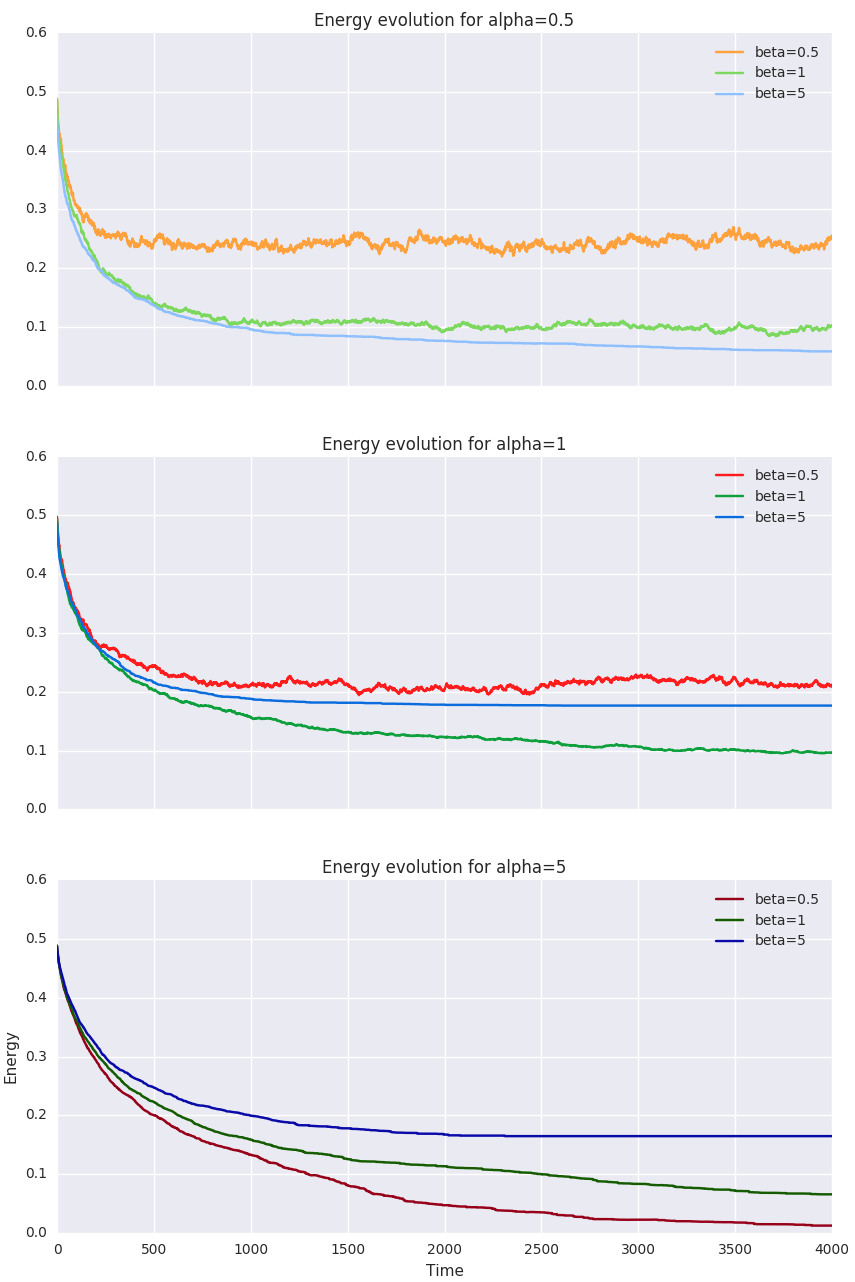
\includegraphics[width=\columnwidth]{../tobekept/ex1_1755923751722050074-r.png}
			\caption{\label{ex1}Évolution de l'énergie en fonction du temps pour divers $\alpha$ et $\beta$}
		\end{figure}
		On peut remarquer sur la \textsc{Figure} \ref{ex1} que pour ces 3 tests avec des valeurs $\alpha$ différentes, le $\beta$ optimal diffère, allant du plus grand pour $\alpha = 0.5$, au plus petit pour $\alpha = 5$.
		Cette valeur optimale nous permet aussi d'obtenir une erreur d'au plus 10\% dans les 3 cas.
		
		\begin{figure}
			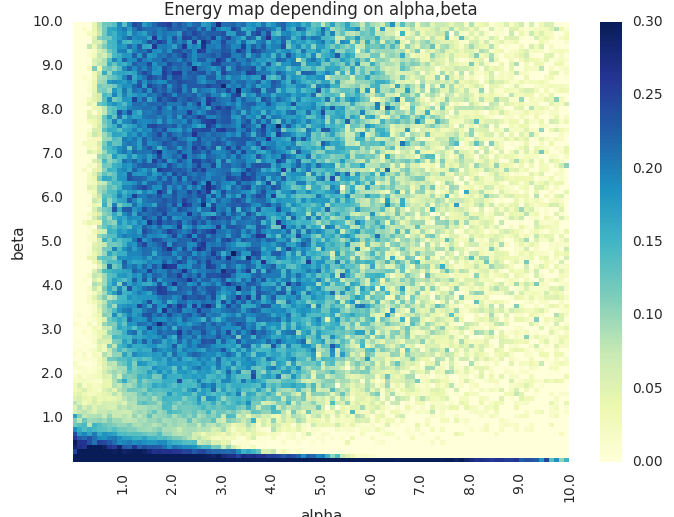
\includegraphics[width=\columnwidth]{../tobekept/ex2_2323132067031870085-r.png}
			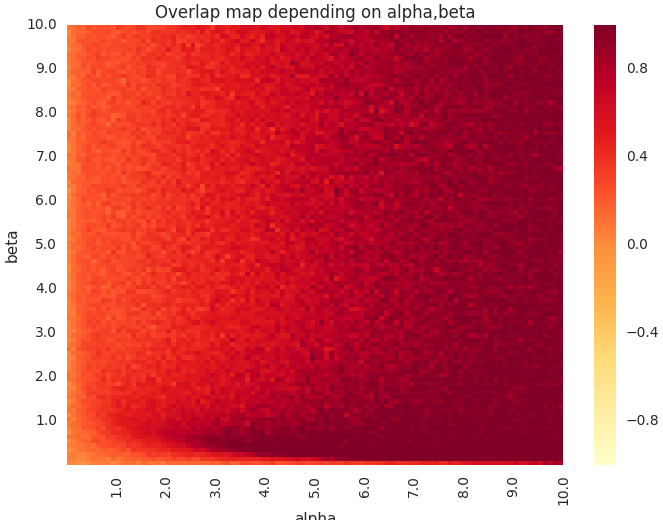
\includegraphics[width=\columnwidth]{../tobekept/ex3_2323132067031870085-r.png}
			\caption{\label{ex2}Représentation de l'énergie et de chevauchement en fonction de $\alpha$ et de $\beta$}
		\end{figure}
		Nous avons réalisé des heat maps décrivant l'énergie et le chevauchement finaux en fonction de $\alpha$ et de $\beta$ (\textsc{Figure} \ref{ex2}). Au regard de ces 2 heat maps, pour de grandes valeurs de $\alpha$, l'énergie est très faible avec de très bons chevauchements. Cependant, on ne voit pas la même tendance pour de faibles $\alpha$ : malgré une énergie faible, le modèle reste assez éloigné de l'original. Comme le nombre de points est plus faible, le modèle est moins bien caractérisé et il semble cohérent que plusieurs modèles parviennent à obtenir une énergie quasi-nulle. 
	\section{Analyse de la valeur de $\beta$}
		La \textsc{Figure} \ref{ex3} représente le meilleur $\beta$ que nous avons pu observer en fonction de $\alpha$. Nous proposons l'approximation : $$\alpha\mapsto\frac{1.5}{\alpha}$$
		À la lumière de ces résultats, nous avons réalisé d'autres graphes de l'évolution de l'énergie en fonction du temps avec des $\beta$ respectant ce modèle. Ils sont en annexe.
	\begin{figure}
		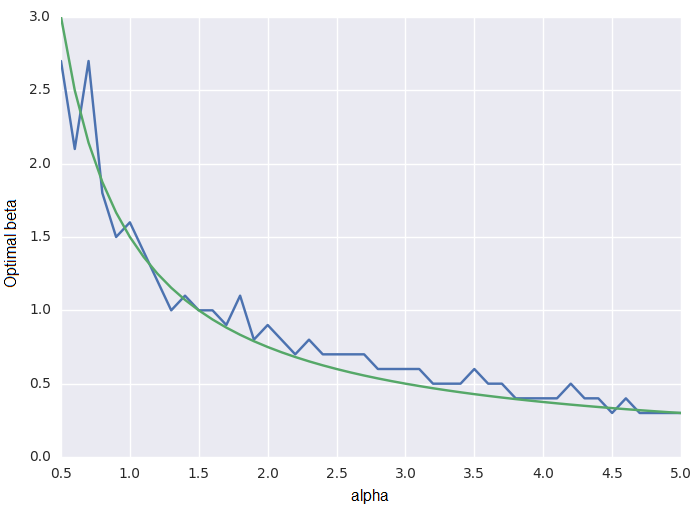
\includegraphics[width=\columnwidth]{../tobekept/exbonus1_2323132067031870085png-r.png}
		\caption{\label{ex3}$\beta$ optimal pour une valeur de $\alpha$ par rapport à $x\mapsto \frac{1.5}{x}$}
	\end{figure}
	\section{Le recuit simulé}
		La méthode du recuit simulé consiste à augmenter progressivement la valeur de $\beta$ au cours de l'algorithme plutôt que de la laisser constante. Dans nos tests, nous avons considéré un $\beta$ initialisé à 0 et un incrément linéaire jusqu'au $\beta$ final.
		On se rend compte en observant les graphes en Annexe que le $\beta$ optimal dépend de $\alpha$.  Nos choix de $\beta$ suivant le modèle proposé précédemment nous donnent de meilleurs résultats qu'avec un $\beta$ constant. Cependant, notre choix pour $\alpha = 1$ semble pouvoir être amélioré.
		
		\begin{figure}
		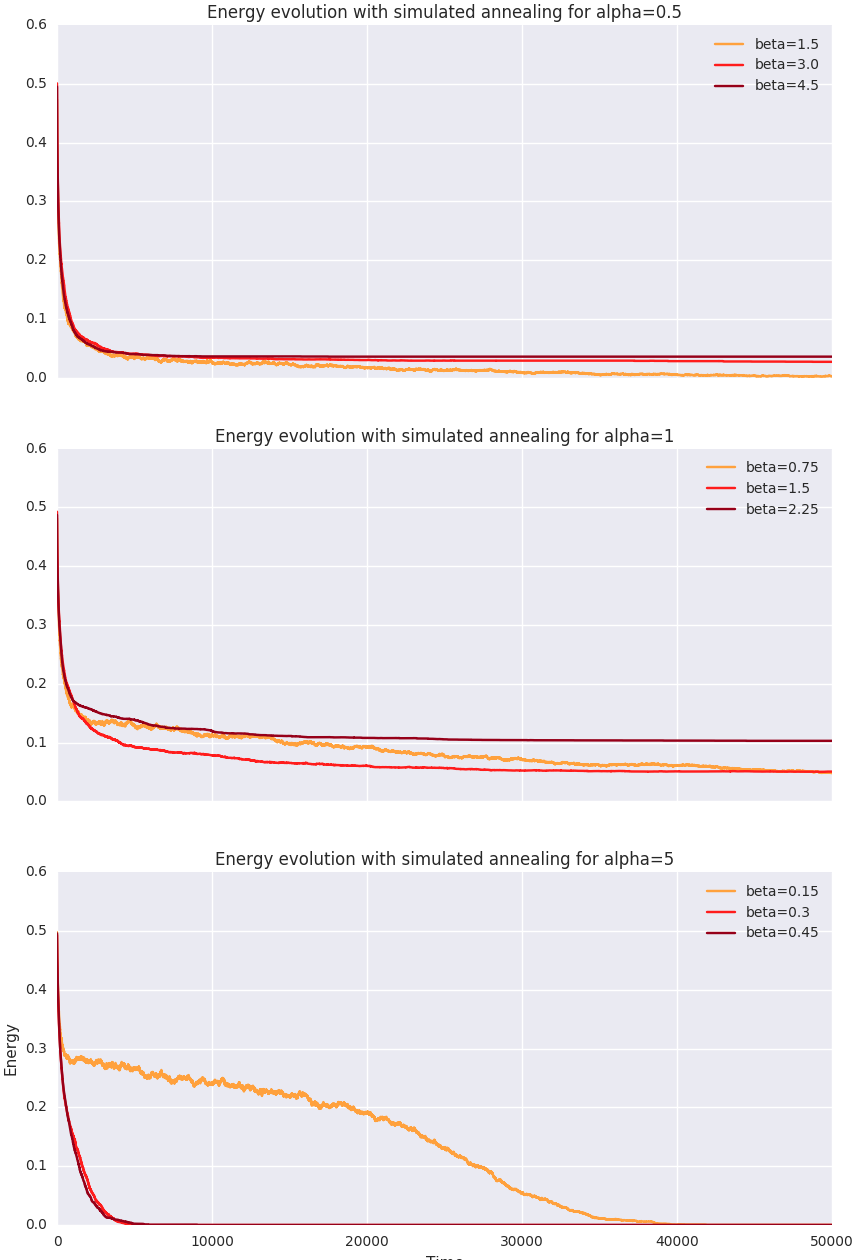
\includegraphics[width=\columnwidth]{../tobekept/ex1_sim_1683536997971113732-r.png}
		\caption{\label{ex1sim}Évolution de l'énergie en fonction du temps pour divers $\alpha$ et $\beta$ avec le recuit simulé}
		\end{figure}
		
	\section{Conclusion}
		De toutes nos observations, il ressort que l'algorithme de Metropolis-Hastings permet d'atteindre un taux de classifications correctes plutôt élevé, et que ce taux est encore plus élevé en utilisant la méthode du recuit simulé.
		
	\section{Pistes d'amélioration}
		Il pourrait être intéressant de changer la manière qu'a la température de diminuer avec le recuit simulé (plutôt que d'augmenter linéairement son inverse).
		
		Par ailleurs, dans la chaîne de Markov étudiée, chaque état a $N$ voisins. Ce nombre de voisins pourrait être augmenté à $2^N-1$ (i.e. travailler sur un graphe complet). Il serait par exemple possible de proposer la modification de $K$ bits à chaque étape, $K$ étant une variable aléatoire. De plus il serait possible de conserver une complexité moyenne en $O(M\cdot(N+T))$ en choisissant par exemple une loi géométrique pour $K$.
		Cela permettrait peut-être d'éviter certains minima locaux.
		
\newpage
\appendix
\section{Annexe 1}
\begin{figure}[!h]
	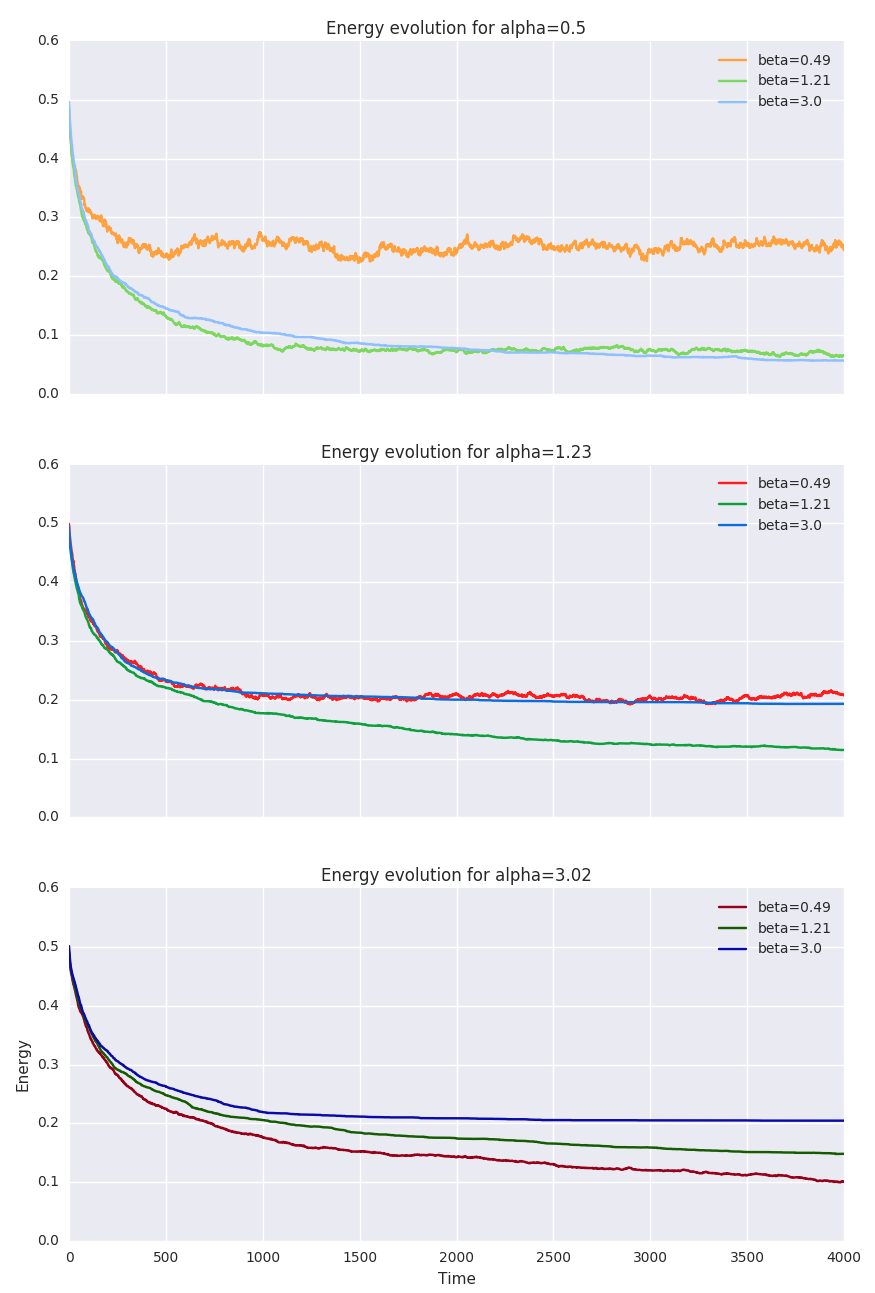
\includegraphics[width=\columnwidth]{../tobekept/ex1_8526750515376798568-r.png}
	\caption{Évolution de l'énergie en fonction du temps pour divers $\alpha$ et les $\beta$ associés ($\frac{1.5}{\alpha}$)}
\end{figure}
\begin{figure}[!h]
	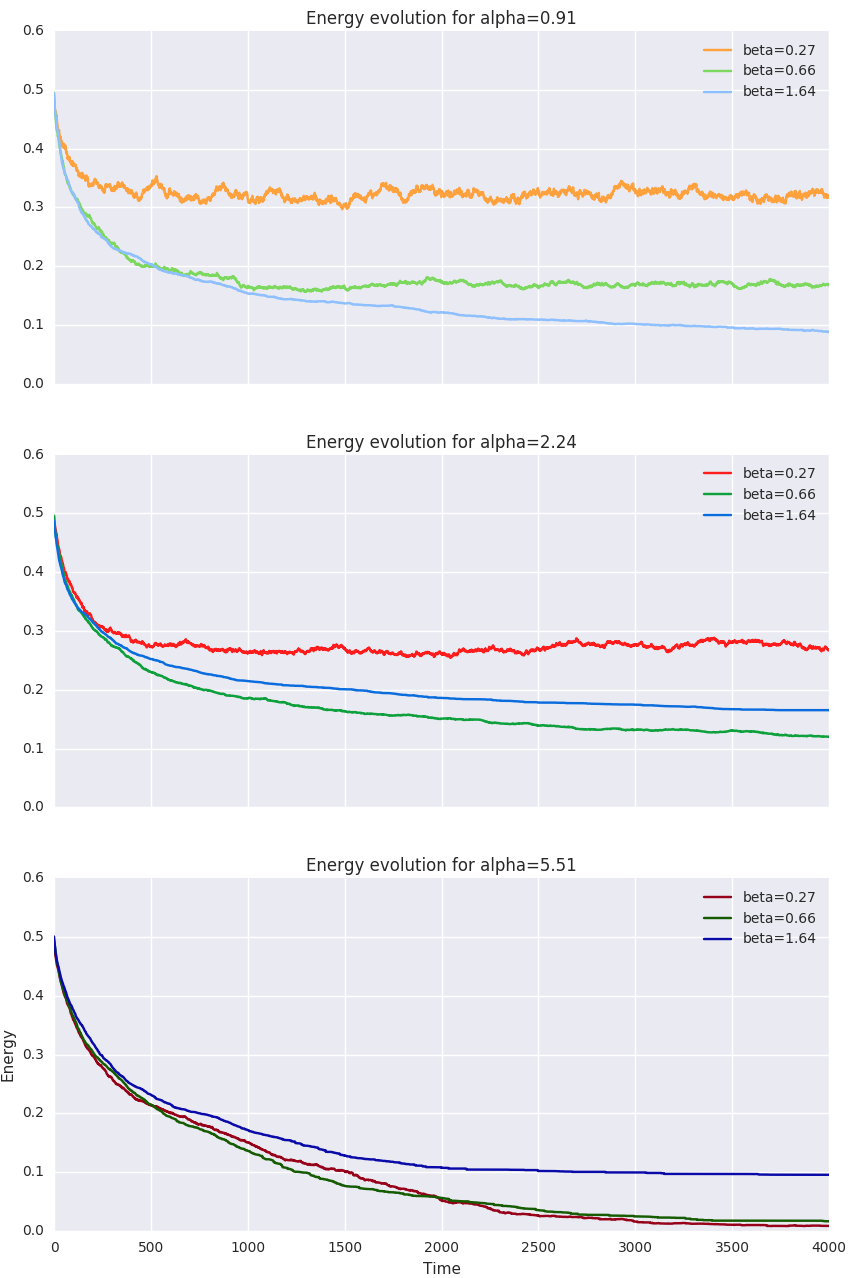
\includegraphics[width=\columnwidth]{../tobekept/ex1_4826864907612068410-r.png}
	\caption{Évolution de l'énergie en fonction du temps pour d'autres $\alpha$ et les $\beta$ associés ($\frac{1.5}{\alpha}$)}
\end{figure}
\clearpage

\section{Annexe 2}
\begin{figure}[!h]
	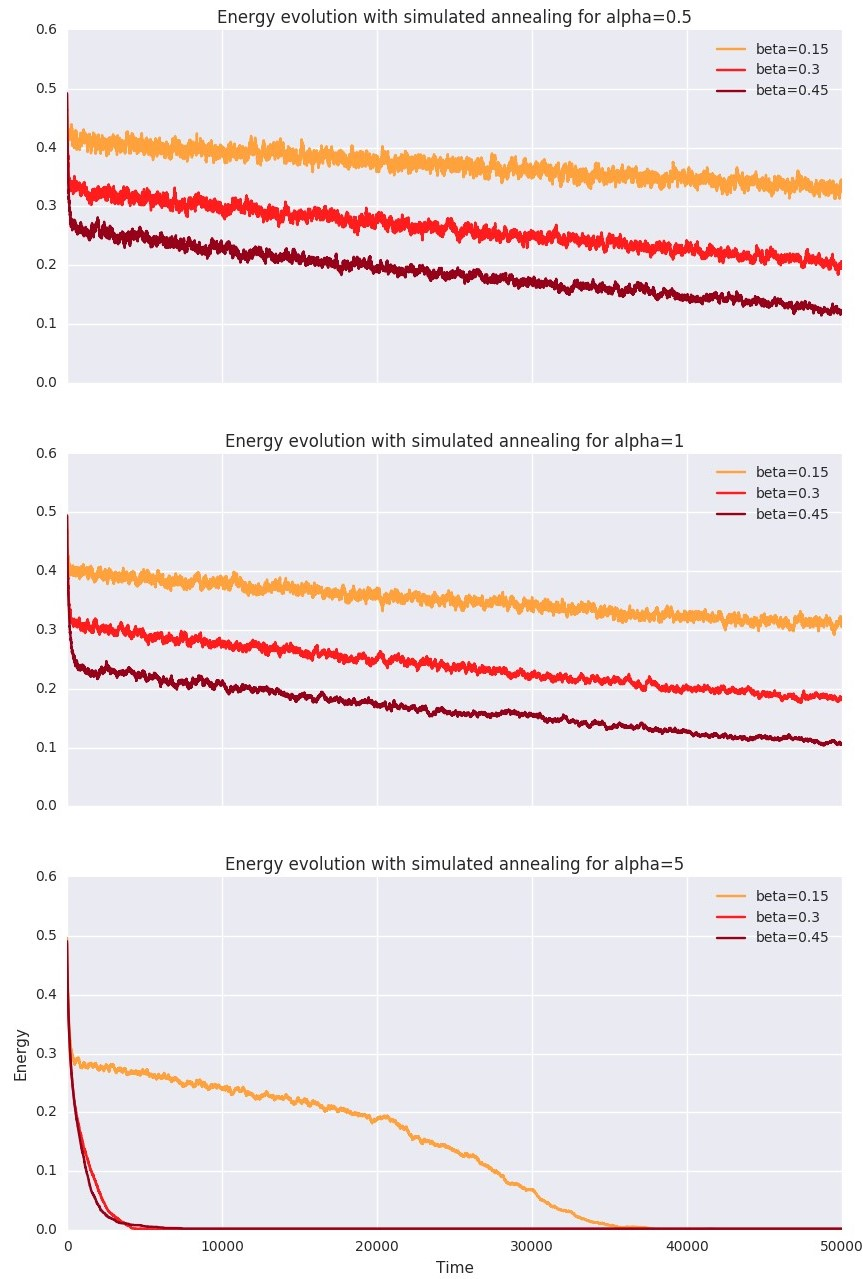
\includegraphics[width=\columnwidth]{../tobekept/skype_1.jpg}
	\caption{Évolution de l'énergie en fonction du temps pour divers $\alpha$ et $\beta$ avec le recuit simulé, avec des $\beta$ trop faibles}
\end{figure}
\begin{figure}[!h]
	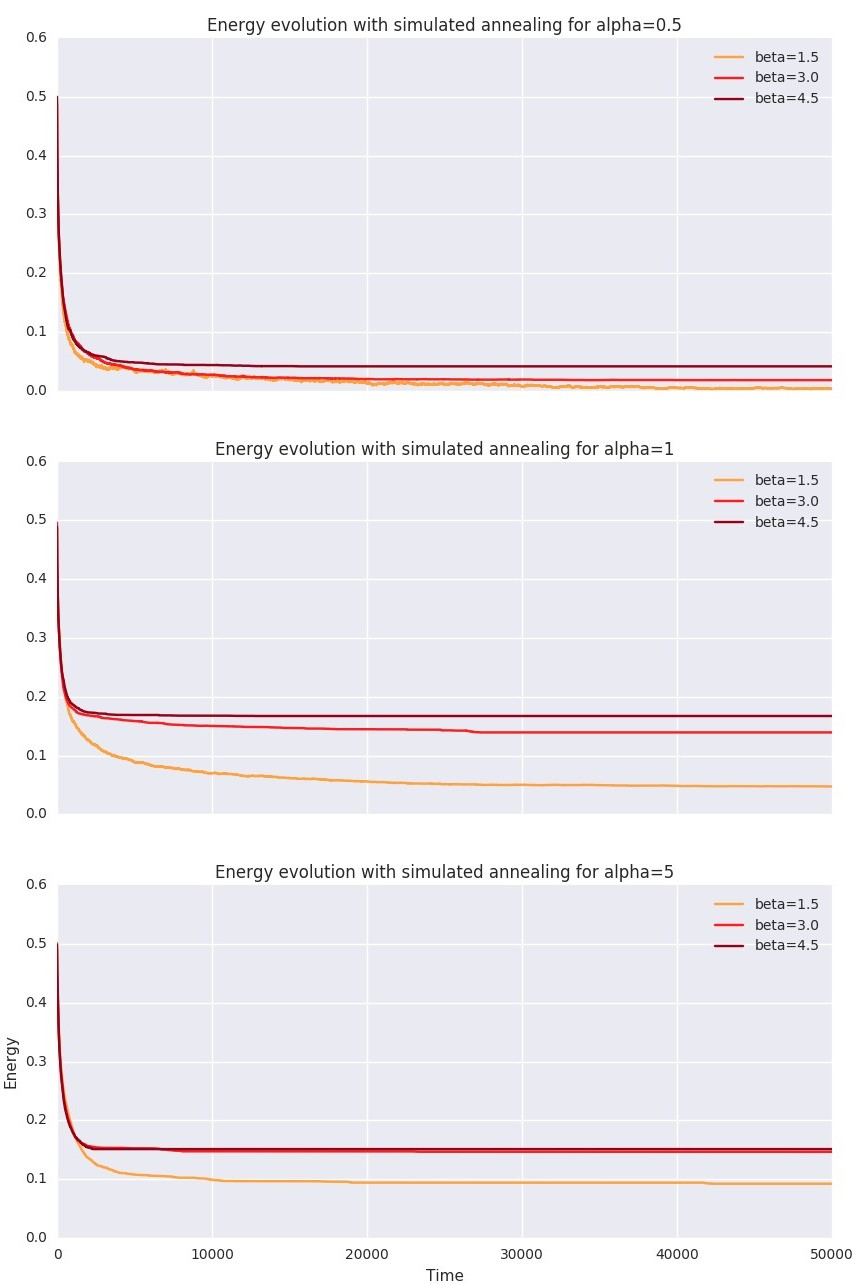
\includegraphics[width=\columnwidth]{../tobekept/skype_2.jpg}
	\caption{Évolution de l'énergie en fonction du temps pour divers $\alpha$ et $\beta$ avec le recuit simulé, avec des $\beta$ trop élevés}
\end{figure}
\end{document}
